% This file is generated by the MATLAB m-file laprint.m. It can be included
% into LaTeX documents using the packages graphicx, color and psfrag.
% It is accompanied by a postscript file. A sample LaTeX file is:
%    \documentclass{article}\usepackage{graphicx,color,psfrag}
%    \begin{document}% This file is generated by the MATLAB m-file laprint.m. It can be included
% into LaTeX documents using the packages graphicx, color and psfrag.
% It is accompanied by a postscript file. A sample LaTeX file is:
%    \documentclass{article}\usepackage{graphicx,color,psfrag}
%    \begin{document}% This file is generated by the MATLAB m-file laprint.m. It can be included
% into LaTeX documents using the packages graphicx, color and psfrag.
% It is accompanied by a postscript file. A sample LaTeX file is:
%    \documentclass{article}\usepackage{graphicx,color,psfrag}
%    \begin{document}% This file is generated by the MATLAB m-file laprint.m. It can be included
% into LaTeX documents using the packages graphicx, color and psfrag.
% It is accompanied by a postscript file. A sample LaTeX file is:
%    \documentclass{article}\usepackage{graphicx,color,psfrag}
%    \begin{document}\input{fig_opt_thr_vs_snr_AWGN}\end{document}
% See http://www.mathworks.de/matlabcentral/fileexchange/loadFile.do?objectId=4638
% for recent versions of laprint.m.
%
% created by:           LaPrint version 3.16 (13.9.2004)
% created on:           22-May-2015 11:17:43
% eps bounding box:     14 cm x 10.5 cm
% comment:              
%
%\begin{psfrags}%
%\psfragscanon%
%
% text strings:
\psfrag{s01}[b][b]{\fontsize{9}{13.5}\fontseries{m}\mathversion{normal}\fontshape{n}\selectfont \color[rgb]{0,0,0}\setlength{\tabcolsep}{0pt}\begin{tabular}{c}$\ers$ = [bits/sec/Hz]\end{tabular}}%
\psfrag{s02}[t][t]{\fontsize{9}{13.5}\fontseries{m}\mathversion{normal}\fontshape{n}\selectfont \color[rgb]{0,0,0}\setlength{\tabcolsep}{0pt}\begin{tabular}{c}$\gamma$ = [dB]\end{tabular}}%
\psfrag{s06}[][]{\fontsize{10}{15}\fontseries{m}\mathversion{normal}\fontshape{n}\selectfont \color[rgb]{0,0,0}\setlength{\tabcolsep}{0pt}\begin{tabular}{c} \end{tabular}}%
\psfrag{s07}[][]{\fontsize{10}{15}\fontseries{m}\mathversion{normal}\fontshape{n}\selectfont \color[rgb]{0,0,0}\setlength{\tabcolsep}{0pt}\begin{tabular}{c} \end{tabular}}%
\psfrag{s08}[l][l]{\fontsize{9}{13.5}\fontseries{m}\mathversion{normal}\fontshape{n}\selectfont \color[rgb]{0,0,0}$\pcd = 0.97$}%
\psfrag{s09}[l][l]{\fontsize{9}{13.5}\fontseries{m}\mathversion{normal}\fontshape{n}\selectfont \color[rgb]{0,0,0}(6)}%
\psfrag{s10}[l][l]{\fontsize{9}{13.5}\fontseries{m}\mathversion{normal}\fontshape{n}\selectfont \color[rgb]{0,0,0}$\pcd = 0.92$}%
\psfrag{s11}[l][l]{\fontsize{9}{13.5}\fontseries{m}\mathversion{normal}\fontshape{n}\selectfont \color[rgb]{0,0,0}$\pcd = 0.95$}%
\psfrag{s12}[l][l]{\fontsize{9}{13.5}\fontseries{m}\mathversion{normal}\fontshape{n}\selectfont \color[rgb]{0,0,0}$\pcd = 0.97$}%
%
% axes font properties:
\fontsize{9}{13.5}\fontseries{m}\mathversion{normal}%
\fontshape{n}\selectfont%
%
% xticklabels:
\psfrag{x01}[t][t]{-15}%
\psfrag{x02}[t][t]{-10}%
\psfrag{x03}[t][t]{-5}%
\psfrag{x04}[t][t]{0}%
\psfrag{x05}[t][t]{5}%
\psfrag{x06}[t][t]{10}%
%
% yticklabels:
\psfrag{v01}[r][r]{1}%
\psfrag{v02}[r][r]{2}%
\psfrag{v03}[r][r]{3}%
\psfrag{v04}[r][r]{4}%
\psfrag{v05}[r][r]{5}%
\psfrag{v06}[r][r]{6}%
\psfrag{v07}[r][r]{7}%
\psfrag{v08}[r][r]{8}%
%
% Figure:
%\resizebox{7cm}{!}{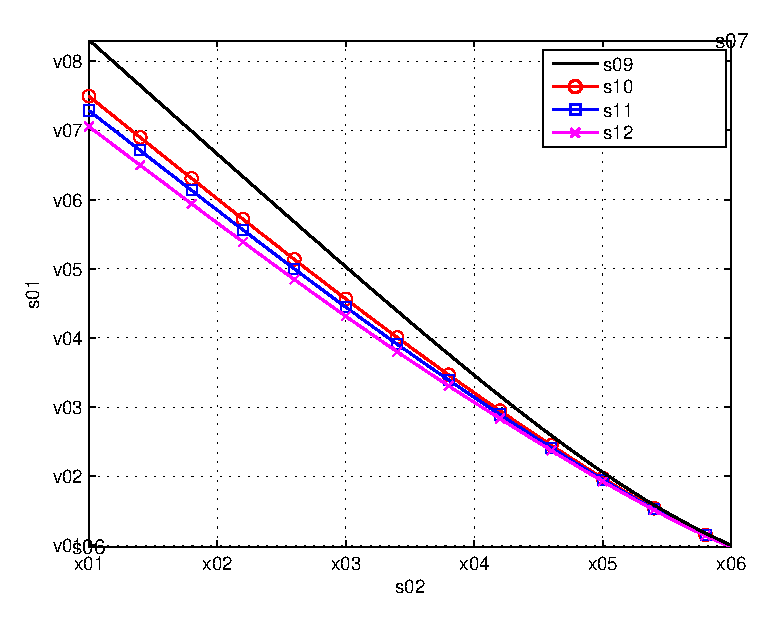
\includegraphics{fig_opt_thr_vs_snr_AWGN.eps}}%
%\end{psfrags}%
%
% End fig_opt_thr_vs_snr_AWGN.tex
\end{document}
% See http://www.mathworks.de/matlabcentral/fileexchange/loadFile.do?objectId=4638
% for recent versions of laprint.m.
%
% created by:           LaPrint version 3.16 (13.9.2004)
% created on:           22-May-2015 11:17:43
% eps bounding box:     14 cm x 10.5 cm
% comment:              
%
%\begin{psfrags}%
%\psfragscanon%
%
% text strings:
\psfrag{s01}[b][b]{\fontsize{9}{13.5}\fontseries{m}\mathversion{normal}\fontshape{n}\selectfont \color[rgb]{0,0,0}\setlength{\tabcolsep}{0pt}\begin{tabular}{c}$\ers$ = [bits/sec/Hz]\end{tabular}}%
\psfrag{s02}[t][t]{\fontsize{9}{13.5}\fontseries{m}\mathversion{normal}\fontshape{n}\selectfont \color[rgb]{0,0,0}\setlength{\tabcolsep}{0pt}\begin{tabular}{c}$\gamma$ = [dB]\end{tabular}}%
\psfrag{s06}[][]{\fontsize{10}{15}\fontseries{m}\mathversion{normal}\fontshape{n}\selectfont \color[rgb]{0,0,0}\setlength{\tabcolsep}{0pt}\begin{tabular}{c} \end{tabular}}%
\psfrag{s07}[][]{\fontsize{10}{15}\fontseries{m}\mathversion{normal}\fontshape{n}\selectfont \color[rgb]{0,0,0}\setlength{\tabcolsep}{0pt}\begin{tabular}{c} \end{tabular}}%
\psfrag{s08}[l][l]{\fontsize{9}{13.5}\fontseries{m}\mathversion{normal}\fontshape{n}\selectfont \color[rgb]{0,0,0}$\pcd = 0.97$}%
\psfrag{s09}[l][l]{\fontsize{9}{13.5}\fontseries{m}\mathversion{normal}\fontshape{n}\selectfont \color[rgb]{0,0,0}(6)}%
\psfrag{s10}[l][l]{\fontsize{9}{13.5}\fontseries{m}\mathversion{normal}\fontshape{n}\selectfont \color[rgb]{0,0,0}$\pcd = 0.92$}%
\psfrag{s11}[l][l]{\fontsize{9}{13.5}\fontseries{m}\mathversion{normal}\fontshape{n}\selectfont \color[rgb]{0,0,0}$\pcd = 0.95$}%
\psfrag{s12}[l][l]{\fontsize{9}{13.5}\fontseries{m}\mathversion{normal}\fontshape{n}\selectfont \color[rgb]{0,0,0}$\pcd = 0.97$}%
%
% axes font properties:
\fontsize{9}{13.5}\fontseries{m}\mathversion{normal}%
\fontshape{n}\selectfont%
%
% xticklabels:
\psfrag{x01}[t][t]{-15}%
\psfrag{x02}[t][t]{-10}%
\psfrag{x03}[t][t]{-5}%
\psfrag{x04}[t][t]{0}%
\psfrag{x05}[t][t]{5}%
\psfrag{x06}[t][t]{10}%
%
% yticklabels:
\psfrag{v01}[r][r]{1}%
\psfrag{v02}[r][r]{2}%
\psfrag{v03}[r][r]{3}%
\psfrag{v04}[r][r]{4}%
\psfrag{v05}[r][r]{5}%
\psfrag{v06}[r][r]{6}%
\psfrag{v07}[r][r]{7}%
\psfrag{v08}[r][r]{8}%
%
% Figure:
%\resizebox{7cm}{!}{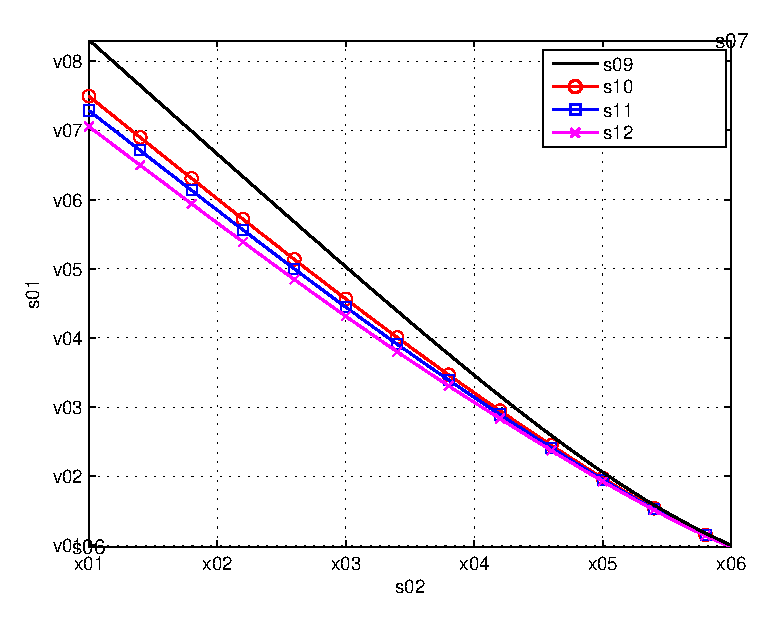
\includegraphics{fig_opt_thr_vs_snr_AWGN.eps}}%
%\end{psfrags}%
%
% End fig_opt_thr_vs_snr_AWGN.tex
\end{document}
% See http://www.mathworks.de/matlabcentral/fileexchange/loadFile.do?objectId=4638
% for recent versions of laprint.m.
%
% created by:           LaPrint version 3.16 (13.9.2004)
% created on:           22-May-2015 11:17:43
% eps bounding box:     14 cm x 10.5 cm
% comment:              
%
%\begin{psfrags}%
%\psfragscanon%
%
% text strings:
\psfrag{s01}[b][b]{\fontsize{9}{13.5}\fontseries{m}\mathversion{normal}\fontshape{n}\selectfont \color[rgb]{0,0,0}\setlength{\tabcolsep}{0pt}\begin{tabular}{c}$\ers$ = [bits/sec/Hz]\end{tabular}}%
\psfrag{s02}[t][t]{\fontsize{9}{13.5}\fontseries{m}\mathversion{normal}\fontshape{n}\selectfont \color[rgb]{0,0,0}\setlength{\tabcolsep}{0pt}\begin{tabular}{c}$\gamma$ = [dB]\end{tabular}}%
\psfrag{s06}[][]{\fontsize{10}{15}\fontseries{m}\mathversion{normal}\fontshape{n}\selectfont \color[rgb]{0,0,0}\setlength{\tabcolsep}{0pt}\begin{tabular}{c} \end{tabular}}%
\psfrag{s07}[][]{\fontsize{10}{15}\fontseries{m}\mathversion{normal}\fontshape{n}\selectfont \color[rgb]{0,0,0}\setlength{\tabcolsep}{0pt}\begin{tabular}{c} \end{tabular}}%
\psfrag{s08}[l][l]{\fontsize{9}{13.5}\fontseries{m}\mathversion{normal}\fontshape{n}\selectfont \color[rgb]{0,0,0}$\pcd = 0.97$}%
\psfrag{s09}[l][l]{\fontsize{9}{13.5}\fontseries{m}\mathversion{normal}\fontshape{n}\selectfont \color[rgb]{0,0,0}(6)}%
\psfrag{s10}[l][l]{\fontsize{9}{13.5}\fontseries{m}\mathversion{normal}\fontshape{n}\selectfont \color[rgb]{0,0,0}$\pcd = 0.92$}%
\psfrag{s11}[l][l]{\fontsize{9}{13.5}\fontseries{m}\mathversion{normal}\fontshape{n}\selectfont \color[rgb]{0,0,0}$\pcd = 0.95$}%
\psfrag{s12}[l][l]{\fontsize{9}{13.5}\fontseries{m}\mathversion{normal}\fontshape{n}\selectfont \color[rgb]{0,0,0}$\pcd = 0.97$}%
%
% axes font properties:
\fontsize{9}{13.5}\fontseries{m}\mathversion{normal}%
\fontshape{n}\selectfont%
%
% xticklabels:
\psfrag{x01}[t][t]{-15}%
\psfrag{x02}[t][t]{-10}%
\psfrag{x03}[t][t]{-5}%
\psfrag{x04}[t][t]{0}%
\psfrag{x05}[t][t]{5}%
\psfrag{x06}[t][t]{10}%
%
% yticklabels:
\psfrag{v01}[r][r]{1}%
\psfrag{v02}[r][r]{2}%
\psfrag{v03}[r][r]{3}%
\psfrag{v04}[r][r]{4}%
\psfrag{v05}[r][r]{5}%
\psfrag{v06}[r][r]{6}%
\psfrag{v07}[r][r]{7}%
\psfrag{v08}[r][r]{8}%
%
% Figure:
%\resizebox{7cm}{!}{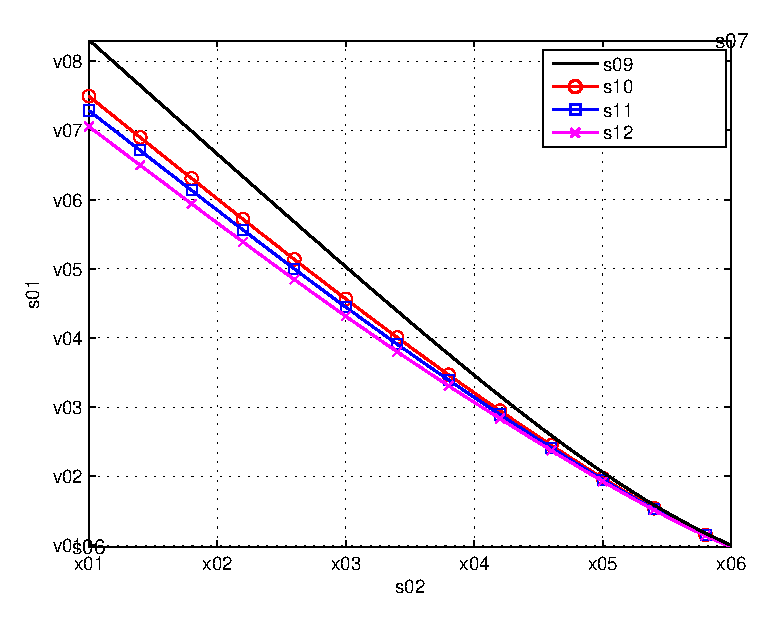
\includegraphics{fig_opt_thr_vs_snr_AWGN.eps}}%
%\end{psfrags}%
%
% End fig_opt_thr_vs_snr_AWGN.tex
\end{document}
% See http://www.mathworks.de/matlabcentral/fileexchange/loadFile.do?objectId=4638
% for recent versions of laprint.m.
%
% created by:           LaPrint version 3.16 (13.9.2004)
% created on:           22-May-2015 11:17:43
% eps bounding box:     14 cm x 10.5 cm
% comment:              
%
%\begin{psfrags}%
%\psfragscanon%
%
% text strings:
\psfrag{s01}[b][b]{\fontsize{9}{13.5}\fontseries{m}\mathversion{normal}\fontshape{n}\selectfont \color[rgb]{0,0,0}\setlength{\tabcolsep}{0pt}\begin{tabular}{c}$\ers$ = [bits/sec/Hz]\end{tabular}}%
\psfrag{s02}[t][t]{\fontsize{9}{13.5}\fontseries{m}\mathversion{normal}\fontshape{n}\selectfont \color[rgb]{0,0,0}\setlength{\tabcolsep}{0pt}\begin{tabular}{c}$\gamma$ = [dB]\end{tabular}}%
\psfrag{s06}[][]{\fontsize{10}{15}\fontseries{m}\mathversion{normal}\fontshape{n}\selectfont \color[rgb]{0,0,0}\setlength{\tabcolsep}{0pt}\begin{tabular}{c} \end{tabular}}%
\psfrag{s07}[][]{\fontsize{10}{15}\fontseries{m}\mathversion{normal}\fontshape{n}\selectfont \color[rgb]{0,0,0}\setlength{\tabcolsep}{0pt}\begin{tabular}{c} \end{tabular}}%
\psfrag{s08}[l][l]{\fontsize{9}{13.5}\fontseries{m}\mathversion{normal}\fontshape{n}\selectfont \color[rgb]{0,0,0}$\pcd = 0.97$}%
\psfrag{s09}[l][l]{\fontsize{9}{13.5}\fontseries{m}\mathversion{normal}\fontshape{n}\selectfont \color[rgb]{0,0,0}(6)}%
\psfrag{s10}[l][l]{\fontsize{9}{13.5}\fontseries{m}\mathversion{normal}\fontshape{n}\selectfont \color[rgb]{0,0,0}$\pcd = 0.92$}%
\psfrag{s11}[l][l]{\fontsize{9}{13.5}\fontseries{m}\mathversion{normal}\fontshape{n}\selectfont \color[rgb]{0,0,0}$\pcd = 0.95$}%
\psfrag{s12}[l][l]{\fontsize{9}{13.5}\fontseries{m}\mathversion{normal}\fontshape{n}\selectfont \color[rgb]{0,0,0}$\pcd = 0.97$}%
%
% axes font properties:
\fontsize{9}{13.5}\fontseries{m}\mathversion{normal}%
\fontshape{n}\selectfont%
%
% xticklabels:
\psfrag{x01}[t][t]{-15}%
\psfrag{x02}[t][t]{-10}%
\psfrag{x03}[t][t]{-5}%
\psfrag{x04}[t][t]{0}%
\psfrag{x05}[t][t]{5}%
\psfrag{x06}[t][t]{10}%
%
% yticklabels:
\psfrag{v01}[r][r]{1}%
\psfrag{v02}[r][r]{2}%
\psfrag{v03}[r][r]{3}%
\psfrag{v04}[r][r]{4}%
\psfrag{v05}[r][r]{5}%
\psfrag{v06}[r][r]{6}%
\psfrag{v07}[r][r]{7}%
\psfrag{v08}[r][r]{8}%
%
% Figure:
%\resizebox{7cm}{!}{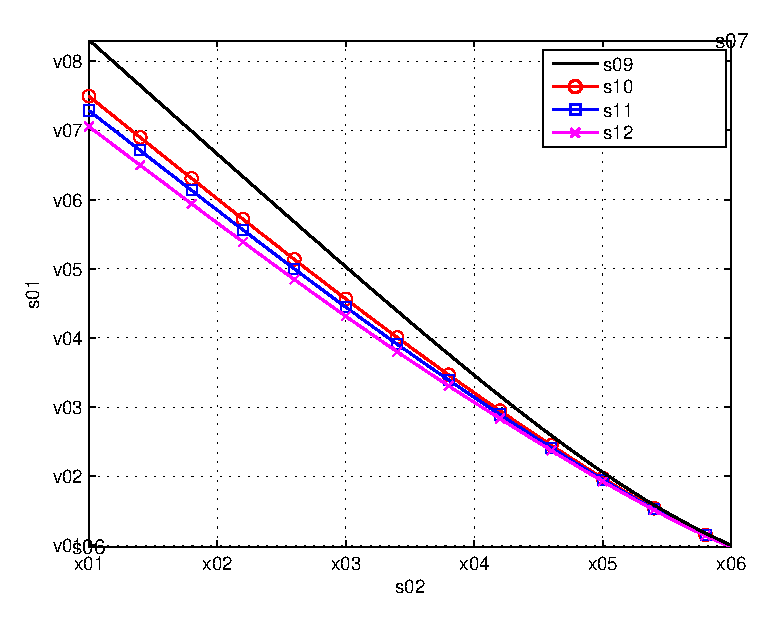
\includegraphics{fig_opt_thr_vs_snr_AWGN.eps}}%
%\end{psfrags}%
%
% End fig_opt_thr_vs_snr_AWGN.tex
